\documentclass[11pt]{article}
\usepackage[a4paper,margin=25mm]{geometry}
\usepackage[T1]{fontenc}
\usepackage{lmodern}
\usepackage{booktabs}
\usepackage{amsmath}
\usepackage{graphicx}
\usepackage{hyperref}
\usepackage{xcolor}
\usepackage{listings}
\lstset{basicstyle=\ttfamily\small, columns=fullflexible, keepspaces=true,
  breaklines=true, frame=single, framerule=0.3pt, rulecolor=\color{gray}}
\newcommand{\code}[1]{\texttt{#1}}
\newcommand{\us}{\textmu s}

\title{\code{chanstat.py}: the 64 channels over many events}
\author{BGOTSCAN}
\date{2026-10-14}

\begin{document}
\maketitle

\section{Purpose}

The single-photoelectron search (\code{template\_doc.tex}) found twelve
channels without any pulse above 20 counts and four channels with five
times the median number, the same four that carry the light in most
events looked at with \code{selection.py}. Dead, low-gain, noisy or hot
channels cannot be told apart on one event. This script accumulates, over
many events of a run, four quantities per channel and shows them as
$8\times8$ maps: the noise, the number of dark-pulse candidates at three
thresholds, how often the channel is lit by scintillation light, and how
much charge it carries when lit. It runs without steps: one table and one
figure at the end. It is a Python script in \code{src/py/}, reading the
raw HDF5 files with h5py; the shared definitions come from the package
\code{bgo} (\code{bgo\_doc.tex}).

\section{Usage}

\begin{lstlisting}
python3 src/py/chanstat.py RUN [options]
\end{lstlisting}

\begin{center}
\begin{tabular}{l l p{76mm}}
\toprule
option & default & meaning \\
\midrule
\code{--data DIR} & the data directory & as in \code{wfview.py} \\
\code{--events SPEC} & \code{0-499} & events to accumulate: \code{a-b} or \code{a,b,c}, 0-based \\
\code{--tail T} & 10 & search region for noise and dark pulses: the last $T$ \us{} of the record \\
\code{--thresholds A,B,C} & \code{12,16,20} & dark-pulse candidate thresholds, in ADC counts \\
\code{--smooth N} & 64 & moving-average width of the pulse search on the sum, in samples \\
\code{--window A,B} & \code{1000,4000} & charge window: ns before and after the maximum of the smoothed sum \\
\code{--nsigma K} & 5 & a channel is lit when its charge exceeds $K$ times its own charge noise \\
\code{--save NAME} & off & save the figure as \code{src/py/plots/NAME\_chanstat.png}; otherwise show it \\
\code{--csv FILE} & off & write the table to \code{FILE} \\
\bottomrule
\end{tabular}
\end{center}

\section{Definitions}

Per event, $x_{c,i} = w_{c,i} - \operatorname{median}_i w_{c,i}$ for every
channel (its own baseline over the record; no common-mode subtraction).
$R$ is the search region, the last $T$~\us{} of the record.

\paragraph{Noise.} $\sigma_c$: the clipped rms of $x_c$ over $R$
(samples beyond three times a first rms are removed, so that pulses do
not inflate it), averaged over events.

\paragraph{Dark-pulse candidates.} $n_c(A)$: the number of local maxima of
the raw $x_c$ inside $R$ above $A$ counts, at least 16 samples apart, for
each threshold $A$ of \code{--thresholds}, summed over events. Below
about 16 counts the candidates are mostly noise maxima; the comparison of
the three thresholds, channel by channel, separates a channel with more
noise (more candidates at every threshold, falling steeply with $A$) from
one with more or larger pulses (more candidates at the high threshold).

\paragraph{Lit channels.} The scintillation pulse is located on the sum
of the 64 channels, smoothed over $N$ samples, at its maximum $i_{\max}$,
and the charge window is $[i_{\max} - a, i_{\max} + b]$
(\code{--window}). The charge of channel $c$ is $q_c = \Delta t \sum_{\rm
window} x_{c,i}$; the control charge $q_c^{\rm ctrl}$ is the same sum
over the last $a + b + 1$ samples of the record (or the first ones if the
window reaches the end). The charge noise of the channel is its own,
$\sigma_{q,c} = \mathrm{rms}$ of $q_c^{\rm ctrl}$ over the events, unlike
\code{selection.py} step~9 which uses one value for all channels. The
channel is lit in an event if $q_c > K \sigma_{q,c}$. The lit fraction
$f_c$ is the number of events where it is lit divided by the number of
events; the mean lit charge $\bar q_c$ is the mean of $q_c$ over those
events.

\section{Output}

\paragraph{Table.} One line per channel: channel, $x$, $y$ (mm, from
\code{src/channel\_map.csv}), $\sigma_c$, $n_c$ at each threshold,
$\sigma_{q,c}$, $f_c$, $\bar q_c$. Below it, the channels that stand out:
$\sigma_c$ more than 20\% from the median; $n_c$ at the highest threshold
above three times or below a third of the median; $f_c$ below a third
of the median (candidates for dead) or above three times it.

\paragraph{Figure.} Four $8\times8$ maps in channel order with the value
printed in each cell: $\sigma_c$; $n_c$ at the highest threshold; $f_c$;
$\bar q_c$. Read together: a dead channel has normal noise, no excess of
candidates, and a lit fraction near zero; a noisy channel has a high
$\sigma_c$ and many candidates at the low thresholds; a hot or high-gain
channel has many candidates at the high threshold and a large $\bar q_c$;
a swapped cable shows as a lit fraction out of place on the map.

\section{Results (2026-10-14)}

\code{195K\_41V\_th20}, 500 events (\code{197K\_39V\_th20} gives the same
picture):

\begin{center}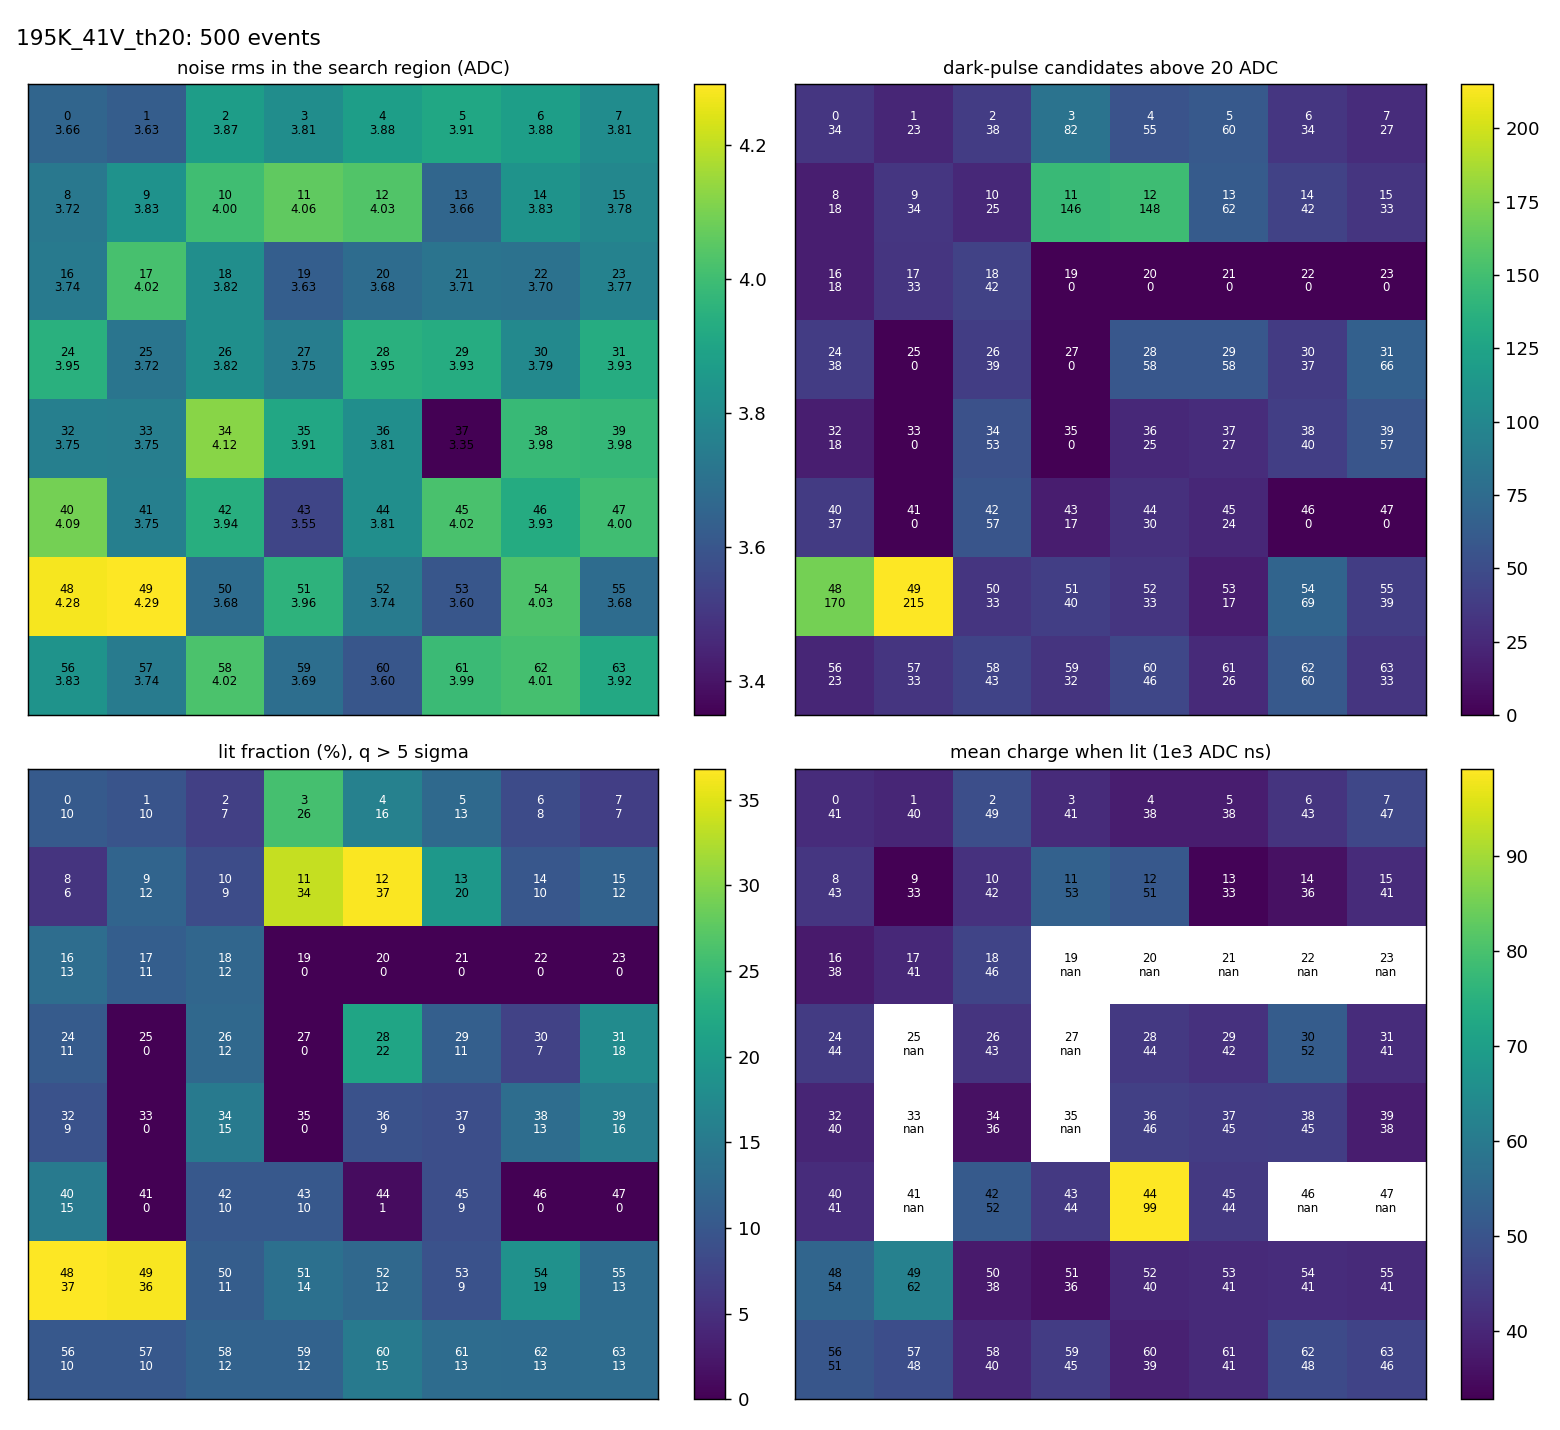
\includegraphics[width=\textwidth]{../figs/chanstat_195K.png}\end{center}

\begin{itemize}
\item \emph{Twelve dead channels}: 19 to 23, 25, 27, 33, 35, 41, 46, 47.
  Normal noise (3.6 to 3.9 counts rms, like every channel), no dark-pulse
  candidate above 16 or 20 counts, lit fraction exactly zero, charge noise
  30\% below the live channels (pure white noise, no pulses). No light
  and no dark counts: no bias or not connected. They form a block on the
  map: the right five of row 2, the pairs 25, 27 and 33, 35 and channel
  41 at the left of rows 3 to 5, and 46, 47 at the right of row 5. That is
  19\% of the face.
\item \emph{Four high-gain channels}: 11, 12, 48, 49. Noise at most 12\%
  above the median, five times the candidates above 20 counts, lit in 34
  to 37\% of the events against a median of 11\%, and a mean charge when
  lit of 51\,000 to 62\,000 ADC\,ns against about 40\,000: 30 to 50\%
  more gain explains all four numbers. The recurring cluster at these
  channels in \code{selection.py} is a gain pattern.
\item \emph{Channel 44}: normal noise and candidates, but a charge noise
  three times the others, lit in 1\% of the events with twice the charge:
  a slow baseline wander. To be watched.
\item The lit fraction of the other 47 channels is flat across the face,
  7 to 20\%, with no edge or row pattern: the source illuminates the
  whole crystal and the map shows nothing wrong.
\end{itemize}

\section{Examples}

\begin{lstlisting}
python3 src/py/chanstat.py 195K_41V_th20 --save cs195
python3 src/py/chanstat.py 197K_39V_th20 --events 0-999 --save cs197 --csv chanstat_197K.csv
\end{lstlisting}

\end{document}
